\section{Hashfunktionen und MACs}
\subsection{Funktionsweise von Hash-Funktionen}

\begin{eqnarray}
	 Y                      & = 11110 \\
	 F:                     & \{0,1\}^4 \rightarrow \{0,1\}^2 ,\\
	 (x_1, x_2, x_3, x_4) & \mapsto (x_1 \xor x_4, x_2 \xor x_3)
\end{eqnarray}

\begin{center}
\begin{tabular}{cc|cc|c}
$x_1$ & $x_2$ & $x_3$ & $x_4$ & $F(x_1,x_2,x_3,x_4)$ \\
$0$ & $0$ & $1$ & $1$ & $11$ \\
$1$ & $1$ & $1$ & $1$ & $00$ \\
$0$ & $0$ & $0$ & $0$ & $00$ \\
\end{tabular}
\end{center}

\subsection{Kollisionen und Preimage-Angriffe}
\[ X = (X_0,X_1,X_2, \ldots , X_{n-1}) \]
\[H(X) = nX_0 + (n - 1)X_1 + (n - 2)X_2 + \ldots +2X_{n−2} + X_{n−1} \mod 256 = \sum\limits_{i\ge 0}^n (n-i)X_i \mod 256 \]
\subsubsection{Berechnen Sie H(X) für die Nachricht "FHT4ever". Interpretieren Sie dabei jeden Buchstaben als seinen 8 Bit ASCII-Wert.}
\begin{align}
X    &= (70, 72, 84, 52, 101, 118, 101, 114) \\
H(X) &= 8 \cdot 70 + 7 \cdot 72 + 6 \cdot 84 + 5 \cdot 52 + 4 \cdot 101 + 3 \cdot 118 + 2 \cdot 101 + 114\\
     &= 560 + 504 + 504 + 260 + 404 + 354 + 202 + 114 \\
     &= 48 + 248 + 248 + 4 + 148 + 98 + 202 + 114     \\
     &= 86
\end{align}

\begin{lstlisting}
H = lambda x: sum([(len(x)-i)*ord(e)\%256 for i,e in enumerate(x)])\%256
\end{lstlisting}

\subsubsection{Finden Sie eine andere (sinnvolle) Nachricht, die den gleichen Hashwert wie "FHT4ever" hat.}

\[  H(Uni4ever) = 86 \]

\subsubsection{Gegeben sei $h(X)=42$, wobei $X = (X_0,X_1,X_2)$. Finden Sie ein $Y =(Y_0,Y_1,Y_2)$ mit $X ≠ Y \wedge
h(Y) = h(X)$.}
\subsubsection{Finden Sie eine weitere Kollision.}


\begin{align}
	H(X) = 42 &= (3 X_1 + 2 X_2 + X_1) \mod 256 	        
\end{align}


Folgende Tabelle gibt Tupeln   $X = (X_0,X_1,X_2)$ mit  $H(X) = 42$ an. 
Insgesamt existieren 65536 Kollision (ExhaustedSearch).
\begin{lstlisting}
	c = [ (x,y,z) for x in range(256) 
                    for y in range(256) 
                      for z in range(256)
                        if (3*x+2*y+z) % 256==42 ]
	print len(c)
\end{lstlisting}
\begin{center}
\begin{tabular}{ccc}
$X_1$&$X_2$&$X_3$\\
96 & 166 & 190 \\
96 & 167 & 188 \\
96 & 168 & 186 
\end{tabular}
\end{center}



\subsection{Das Online-Auktionshaus}

\subsubsection{Denken Sie sich ein möglichst einfaches Verfahren aus, das auf einer Hash-Funktion beruht.}

Ein Gebot ist ein Hashwert bestehend aus: Betrage, Timestamp und Nonce $$H(( bid \circ time \circ salt) ) = Y$$
Die anderen Bieter können nicht errechnen welchen Betrag ein Bieter geboten hat,
da die Umkehrung von $H$ nicht möglich ist.

Sobald die Bieterrunde geschlossen wird, schickt jeder Bieter sein Gebot, Timestamp und Nonce zum Auktionator. 
Dieser kann nun die Hashwerte der Gebote überprüfen und den günstigen Bieter ermitteln.

Folgendes Bild zeigt ein Beispielablauf einer Auktion.

\begin{center}
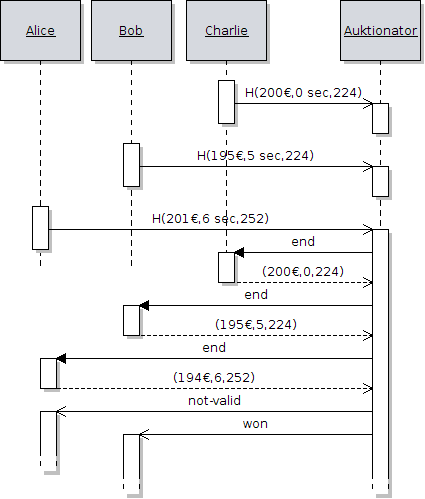
\includegraphics[scale=0.5]{images/auction-bidding.png}
\end{center}

Im Beispiel sehen, dass Alices Gebot abgelehnt wird da $$H(  201 \circ \ldots  ) = H( 196 \circ \ldots)$$
Sowie das Bob gewinnt, da er das günstigste Gebot abgeben hat.

\subsubsection{Welche Angriffe gibt es trotzdem noch auf das Verfahren?}

\begin{itemize}
\item Man-in-the-Middle Attake aufgrund fehlender Authentizität.
\item Störungen des Übertragungskanals
\item ohne Timetamp wäre Replayangriffe möglich
\item ohne Salt wäre die Authentifizierung komplett ausgehebelt
\end{itemize}

\subsection{Datenbankschutz durch Verschlüsselung und Hash-Funktionen}

\lstset{language=SQL}
\lstinputlisting{eclipse/member.db.sql}



\subsection{kryptologische Absicherung der Prüfungsvorleistung}
\subsubsection{Das Verfahren ist bisher kryptologisch nicht gesichert. Welche Angriffe sind denkbar?}
\begin{itemize}
\item Identitätsdiebstahl, man verwendet den Zettel eines anderen
\item Replikation des eigenen Scheines mit Fälschung des Ergebnisses
\item Replikation eines anderen Scheines Fälschung der persönlichen Angaben
\end{itemize}

\subsubsection{Sichern Sie das Verfahren kryptologisch ab. 
               Der Professor soll die "Echtheit" der Bescheinigung möglichst einfach prüfen können.}
               
(1) Auf dem Schein wird ein QR-Code abgedruckt der einen Hash mit den Angaben auf dem Schein und einen geheimen Saltwert beinhaltet. Dies kann mit einem Handy leicht geprüft. Überprüfung der Identität ist weiterhin erforderlich.

(2) Verfahren (1) kann auch als Hex-Zeichen aufgedruckt werden.

(3) $H(Matrikel,Bestanden,Salt) = (Matrikel+Bestanden+Salt \mod N)$